In order to select either the PLM or the IM-II, a symmetry based framework in four steps was implemented. This framework initially proposed in \cite{ohlsson2020symmetry} consists of the following four steps:

\begin{enumerate}
\item Transform the original time series using the symmetry of interest,
\item Fit the candidate model to the transformed time series,
\item Inversely transform the model back,
\item Compare the inversely transformed model to the original time series.
\end{enumerate}

The idea behind the above steps is that if a symmetry is manifest in the original data then the fit will be invariant under transformations by the symmetry. This implies that for a model with a symmetry that is manifest in the data, the fit of the inversely transformed model to the original data will be the same as the fit of the original model to the original data. Conversely, if a symmetry is \textit{not} manifest in the data then the symmetry will distort the data as it is transformed which will \textit{decrease} the fit of the candidate model. This effect will get more pronounced the longer the data and the candidate models are transformed using the symmetry. A measure of this effect is the so called \textit{relative RMS} denoted by $\Delta(\epsilon)$ \cite{ohlsson2020symmetry} which is defined as follows

\begin{equation}
\Delta(\epsilon)=\dfrac{\rho(\epsilon)}{\rho_{0}}-1.
  \label{eq:model_selection}
\end{equation}
Here, $\rho_{0}=\mathrm{RMS}$ is the fit in terms of the root mean square of the original curve to the original data and $\rho(\epsilon)$ is the fit in terms of the RMS of the inversely transformed model to the original data when the model selection framework above is implemented with a transformation parameter $\epsilon$. If a symmetry is manifest in the data meaning that the fitting of the model to the data is invariant under the action of the symmetry, then $\rho(\epsilon)\approx \rho_{0}$ implying that $\Delta(\epsilon)\approx 0$. On the other hand, if the symmetry of the candidate model is not manifest in the data then $\rho(\epsilon)> \rho_{0}$ and thus $\Delta(\epsilon)>0$ where it is expected that $\Delta(\epsilon)$ increases with an increasing $\epsilon$ as the fit will get worse the more the data as well as the candidate model are transformed.

For illustration purposes, this framework has been implemented for the $t$-directional symmetries of the PLM  and the IM-II. When implementing this framework of the $t$-directional scaling symmetry $\Gamma_{1,1}(\epsilon)$ of the PLM with a parameter of $\epsilon=0.2$, the conclusion is that this symmetry is indeed manifest in the data (Fig \ref{fig:model_sel_PLM}). In contrast, the $t$-directional symmetry $\Gamma_{2}(\epsilon)$ of the IM-II is not manifest in the data illustrated by the implementation of the symmetry based framework for model selection with a transformation parameter of $\epsilon=7$ (Fig \ref{fig:model_sel_IM_II}). 







\begin{figure}[htbp!]
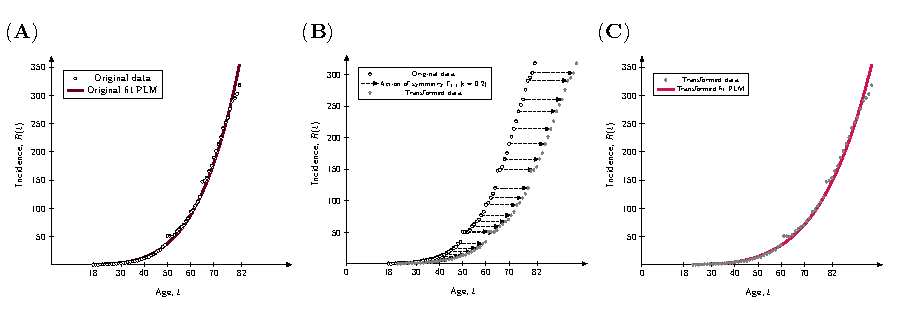
\includegraphics[width=\textwidth]{FigS6.pdf}
\caption[Illustration of the model selection framework for the PLM]{\textit{Illustration of the model selection framework for the PLM}. The symmetry based framework using the $t$-directional scaling symmetry $\Gamma_{1,1}$ of the PLM. The framework illustrates that this symmetry is indeed manifest in the data and the model selection is conducted in four steps. (\textbf{A}) The original time series in the black circles is transformed using the scaling symmetry $\Gamma_{1,1}$ with a transformation parameter of $\epsilon=0.2$ in order to produce a transformed time series illustrated in the grey diamonds. (\textbf{B}) The PLM is fitted to the transformed time series. (\textbf{C}) The fitted model is inversely transformed with a transformation parameter of $\epsilon=0.2$ by the inverse transformation defined by $\Gamma^{-1}_{1,1}(\epsilon)=\Gamma_{1,1}(-\epsilon)$. (\textbf{D}) The fit of the inversely transformed model is compared to the original time series. The family of PLM curves illustrated in the figure are generated by the parameter $\gamma=4.528$ and the curves as well as the data is transformed with a transformation parameter of $\epsilon=0.2$.}
\label{fig:model_sel_PLM}
\end{figure}












\begin{figure}[htbp!]
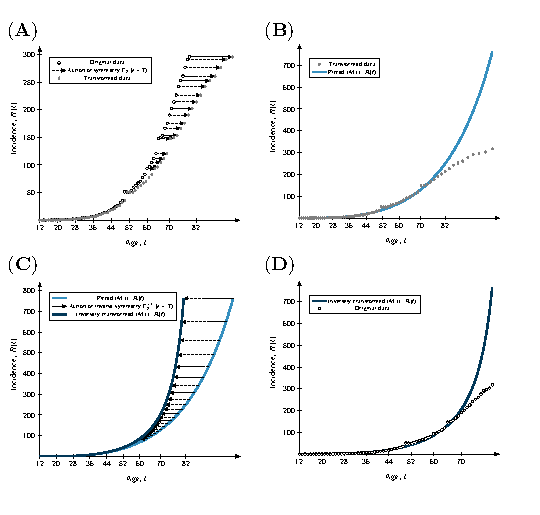
\includegraphics[width=\textwidth]{FigS7.pdf}
\caption[Illustration of the model selection framework for the IM-II]{\textit{Illustration of the model selection framework for the IM-II}. The symmetry based framework using the $t$-directional symmetry $\Gamma_{2}$ of the IM-II. The framework illustrates that this symmetry is \textit{not} manifest in the data and the model selection is conducted in four steps. (\textbf{A}) The original time series in the black circles is transformed using the scaling symmetry $\Gamma_{2}$ with a transformation parameter of $\epsilon=7$ in order to produce a transformed time series illustrated in the grey diamonds. (\textbf{B}) The IM-II is fitted to the transformed time series. (\textbf{C}) The fitted model is inversely transformed with a transformation parameter of $\epsilon=7$ by the inverse transformation defined by $\Gamma^{-1}_{2}(\epsilon)=\Gamma_{2}(-\epsilon)$. (\textbf{D}) The fit of the inversely transformed model is compared to the original time series. The family of IM-II curves illustrated in the figure are generated by the parameters $(\tau,\alpha)=(58.378,0.044)$ and the curves as well as the data is transformed with a transformation parameter of $\epsilon=0.2$.}
\label{fig:model_sel_IM_II}
\end{figure}